{Given the graph of $f$, identify the concavity of $f$ and its inflection points.\\
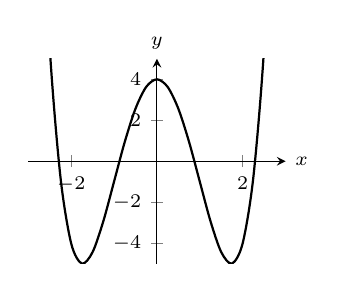
\begin{tikzpicture}
\begin{axis}[width=.4\textwidth,tick label style={font=\scriptsize },
	axis y line=middle,axis x line=middle,
    ymin=-5,ymax=5,
	xmin=-3,xmax=3,name=myplot]
\addplot [{\colorone},smooth,thick,domain=-3:3] {x^2*(x^2-6)+4};
\end{axis}
\node [right] at (myplot.right of origin) {\scriptsize $x$};
\node [above] at (myplot.above origin) {\scriptsize $y$};
\end{tikzpicture}
}
{concave up on $(-\infty,-1)\cup(1,\infty)$;\\
concave down on $(-1,1)$;\\
inflection points when $x=\pm1$}
